% Vietnamese translation for OI Public Library
% Source-PDF: IOI中国国家候选队论文/1999/邵铮.pdf
\documentclass[11pt]{article}
\usepackage{tikz}
\usetikzlibrary{calc}
\usepackage{oipl-vn}

\newcommand{\pentagonstate}[4]{%
  \begin{scope}[shift={(#1,#2)}]
    \coordinate (p1) at (90:0.42);
    \coordinate (p2) at (18:0.42);
    \coordinate (p3) at (-54:0.42);
    \coordinate (p4) at (-126:0.42);
    \coordinate (p5) at (162:0.42);
    \draw (p1)--(p2)--(p3)--(p4)--(p5)--cycle;
    \node[font=\tiny] at ($(p1)+(0,0.16)$) {1};
    \node[font=\tiny] at ($(p2)+(0.16,0.02)$) {2};
    \node[font=\tiny] at ($(p3)+(0.10,-0.14)$) {3};
    \node[font=\tiny] at ($(p4)+(-0.10,-0.14)$) {4};
    \node[font=\tiny] at ($(p5)+(-0.16,0.02)$) {5};
    #3
    \node[font=\scriptsize] at (0,-0.68) {#4};
  \end{scope}%
}

\title{Xây dựng, so sánh và ứng dụng mô hình toán học}
\author{Shao Zheng}
\date{}

\begin{document}
\maketitle

\origtitle{Establishment, comparison, and application of mathematical models}
\sourcepath{IOI China candidate team papers / 1999 / Shao Zheng.pdf}

\paragraph{Từ khóa.}
Mô hình toán học; thuật toán; hàm sinh.

\section*{Tóm tắt}

Mô hình toán học là một công cụ cơ bản để giải quyết các vấn đề thực tế. Trừu
tượng hóa một vấn đề thực tế thành một mô hình toán học, dùng công cụ toán
học để giải mô hình ấy, rồi áp dụng kết quả cho cả một lớp bài toán có cùng
đặc trưng, là một con đường cơ bản để giải bài. Bài viết trước hết giới thiệu
một số tính chất của mô hình toán học; sau đó xây dựng ba mô hình toán học
khác nhau để giải cùng một bài toán, so sánh chúng để rút ra quan hệ giữa mức
độ trừu tượng và hiệu quả của mô hình; tiếp đó mở rộng mô hình sang hai bài
toán khác để rút ra quan hệ giữa mức độ trừu tượng và khả năng khái quát; cuối
cùng tổng kết toàn văn và nêu một số quy luật chung về mô hình toán học.

\section{Dẫn nhập}

Các vấn đề thực tế thường rối rắm và phức tạp, còn quy luật bên trong lại bị
che giấu. Muốn dùng máy tính trực tiếp giải các vấn đề thực tế thường sẽ gặp
khó khăn nhất định. Điều mà máy tính giỏi xử lý là các vấn đề toán học. Vì
vậy, ta cần trừu tượng hóa vấn đề thực tế thành mô hình toán học, rồi dùng
máy tính để giải mô hình ấy.

So với vấn đề thực tế, mô hình toán học có các tính chất sau.

\begin{enumerate}
  \item \term{Tính trừu tượng.} Mô hình toán học là một dạng trừu tượng hóa
  của vấn đề thực tế. Nó loại bỏ những phần không liên quan đến việc giải bài
  và thể hiện ngắn gọn bản chất của vấn đề. Đây là cơ sở của hai tính chất
  tiếp theo.

  \item \term{Tính hiệu quả.} Quan hệ giữa các đại lượng trong mô hình toán
  học rõ ràng hơn, nên dễ tìm ra quy luật và nhờ đó nâng cao hiệu quả giải.
  Vì tính chất này do tính trừu tượng của mô hình quyết định, mức độ trừu
  tượng hóa có ảnh hưởng quan trọng đến hiệu quả của mô hình. Điều này sẽ
  được trình bày chi tiết trong phần thứ hai.

  \item \term{Tính khái quát.} Mô hình toán học có thể được mở rộng cho cả
  một lớp vấn đề có cùng tính chất. Nói cách khác, giải được một mô hình toán
  học tức là giải được một lớp vấn đề thực tế. Ở đây, ``cùng tính chất'' nghĩa
  là cùng bản chất; những vấn đề nhìn bề ngoài dường như hoàn toàn không liên
  quan vẫn có thể có cùng bản chất. Vì tính chất này cũng do tính trừu tượng
  của mô hình quyết định, mức độ trừu tượng hóa có ảnh hưởng quan trọng đến
  phạm vi khái quát của mô hình. Điều này sẽ được trình bày chi tiết trong
  phần thứ ba.
\end{enumerate}

\section{Xây dựng và so sánh mô hình toán học}

Do góc nhìn khác nhau, trước cùng một vấn đề thực tế ta có thể xây dựng nhiều
mô hình toán học khác nhau. Trong các mô hình ấy, điều ta cần tìm là mô hình
có hiệu quả cao. Hiệu quả của mô hình liên quan đến mức độ trừu tượng hóa của
nó. Sau đây ta phân tích quan hệ cụ thể ấy qua một ví dụ.

\paragraph{Bài toán chia đa giác.}
Chia một đa giác lồi \(n\) cạnh bằng \(n-3\) đường chéo đôi một không cắt nhau
thành \(n-2\) tam giác. Hỏi tổng số phương án chia là bao nhiêu?

Chẳng hạn, khi \(n=5\), có năm phương án chia, tương ứng với năm cách chọn hai
đường chéo không cắt nhau để tam giác hóa ngũ giác lồi.

Bài toán này có thể được giải bằng vài phương pháp sau.

\subsection{Phương pháp tìm kiếm}

Ý tưởng của phương pháp này là liệt kê toàn bộ các phương án chia.

Rõ ràng, một tập gồm \(n-3\) đường chéo đôi một không cắt nhau tương ứng với
một phương án chia. Vì vậy, có thể xem bài toán là bài toán đếm số nhóm đường
chéo khác nhau.

Đánh số \(n\) đỉnh của đa giác \(n\) cạnh theo chiều kim đồng hồ là
\(1,2,3,\ldots,n\). Một đường chéo có thể được biểu diễn bởi cặp số
\((a_1,a_2)\), trong đó \(a_1,a_2\) lần lượt là số hiệu hai đỉnh đầu mút,
\(a_1<a_2\), \(a_1\) là đầu đầu và \(a_2\) là đầu cuối của đường chéo.

Thứ tự các đường chéo trong một nhóm là không quan trọng, nên một nhóm đường
chéo là một tập hợp mà các phần tử là đường chéo.

Một vấn đề bắt buộc phải giải quyết là kiểm tra hai đường chéo có cắt nhau
hay không. Giả sử hai đường chéo lần lượt là \((a_1,a_2)\) và \((b_1,b_2)\).
Nếu xem cặp số biểu diễn đường chéo như một khoảng mở, thì điều kiện cần và
đủ để hai đường chéo không cắt nhau là hai khoảng ấy có quan hệ chứa nhau hoặc
giao của chúng rỗng.

Như vậy, ta xây dựng mô hình toán học đầu tiên cho bài toán này:
\begin{quote}
Biết giá trị \(n\).

Một tập hợp gồm \(n-3\) khoảng mở khác nhau \((i,j)\), trong đó
\[
  i\in\{1,\ldots,n-2\},\qquad
  j\in\{i+2,\ldots,n\},
\]
và \((i\ne 1)\) hoặc \((j\ne n)\).

Với hai khoảng mở khác nhau bất kỳ \((i_1,j_1)\), \((i_2,j_2)\) trong cùng
một tập, ta có
\[
  (i_1,j_1)\cap(i_2,j_2)=\varnothing,
\]
hoặc \((i_1,j_1)\) chứa \((i_2,j_2)\), hoặc \((i_2,j_2)\) chứa
\((i_1,j_1)\).

Cần tìm số tập hợp khác nhau.
\end{quote}

Khi tìm kiếm, trước hết xét các đường chéo có đỉnh \(1\) làm đầu đầu: có thể
không nối đường chéo nào, có thể nối \((1,3)\), có thể nối \((1,4)\), hoặc
đồng thời nối \((1,3)\) và \((1,4)\). Với mỗi trường hợp, lại xét các đường
chéo có đỉnh \(2\) làm đầu đầu, rồi tiếp tục như vậy. Khi thu được \(n-3\)
đường chéo đôi một không cắt nhau, ta tìm được một phương án.

Hình dưới phục dựng cây tìm kiếm cho trường hợp
\(n=5\): mỗi nhánh biểu diễn việc chọn hoặc bỏ qua một đường chéo đang xét;
các lá được đánh dấu là những phương án chia khác nhau.

\begin{center}
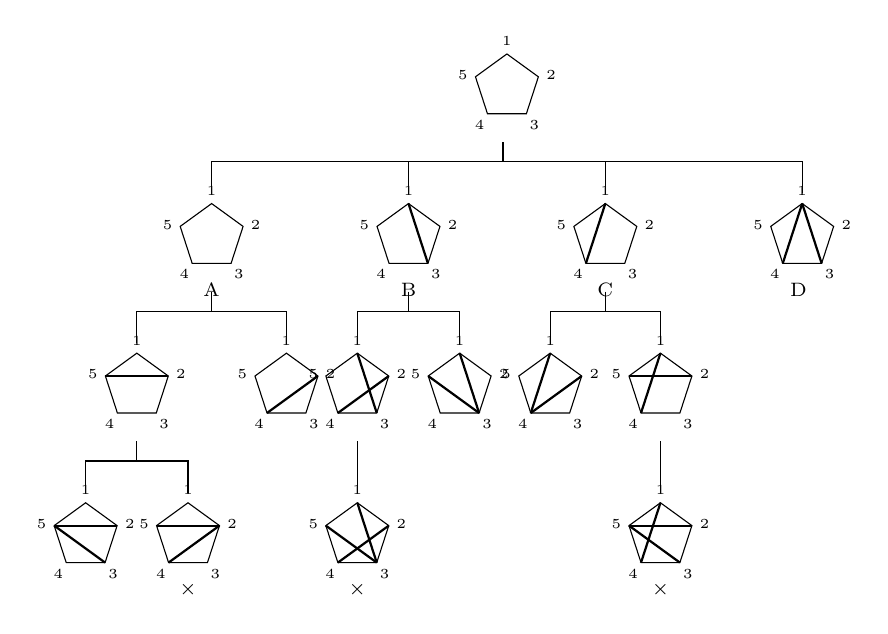
\begin{tikzpicture}[x=1cm,y=1cm,every node/.style={font=\scriptsize}]
  \pentagonstate{0}{3.8}{}{ }
  \draw (-0.05,3.1) -- (-0.05,2.85) -- (-3.75,2.85) -- (-3.75,2.45);
  \draw (-0.05,2.85) -- (-1.25,2.85) -- (-1.25,2.45);
  \draw (-0.05,2.85) -- (1.25,2.85) -- (1.25,2.45);
  \draw (-0.05,2.85) -- (3.75,2.85) -- (3.75,2.45);

  \pentagonstate{-3.75}{1.9}{}{A}
  \pentagonstate{-1.25}{1.9}{\draw[thick] (p1)--(p3);}{B}
  \pentagonstate{1.25}{1.9}{\draw[thick] (p1)--(p4);}{C}
  \pentagonstate{3.75}{1.9}{\draw[thick] (p1)--(p3);\draw[thick] (p1)--(p4);}{D \(\checkmark\)}

  \draw (-3.75,1.2) -- (-3.75,0.95) -- (-4.7,0.95) -- (-4.7,0.55);
  \draw (-3.75,0.95) -- (-2.8,0.95) -- (-2.8,0.55);
  \pentagonstate{-4.7}{0.0}{\draw[thick] (p2)--(p5);}{}
  \pentagonstate{-2.8}{0.0}{\draw[thick] (p2)--(p4);}{\(\checkmark\)}
  \draw (-4.7,-0.7) -- (-4.7,-0.95) -- (-5.35,-0.95) -- (-5.35,-1.35);
  \draw (-4.7,-0.95) -- (-4.05,-0.95) -- (-4.05,-1.35);
  \pentagonstate{-5.35}{-1.9}{\draw[thick] (p2)--(p5);\draw[thick] (p3)--(p5);}{}
  \pentagonstate{-4.05}{-1.9}{\draw[thick] (p2)--(p5);\draw[thick] (p2)--(p4);}{\(\times\)}

  \draw (-1.25,1.2) -- (-1.25,0.95) -- (-1.9,0.95) -- (-1.9,0.55);
  \draw (-1.25,0.95) -- (-0.6,0.95) -- (-0.6,0.55);
  \pentagonstate{-1.9}{0.0}{\draw[thick] (p1)--(p3);\draw[thick] (p2)--(p4);}{}
  \pentagonstate{-0.6}{0.0}{\draw[thick] (p1)--(p3);\draw[thick] (p3)--(p5);}{\(\checkmark\)}
  \draw (-1.9,-0.7) -- (-1.9,-0.95) -- (-1.9,-1.35);
  \pentagonstate{-1.9}{-1.9}{\draw[thick] (p1)--(p3);\draw[thick] (p2)--(p4);\draw[thick] (p3)--(p5);}{\(\times\)}

  \draw (1.25,1.2) -- (1.25,0.95) -- (0.55,0.95) -- (0.55,0.55);
  \draw (1.25,0.95) -- (1.95,0.95) -- (1.95,0.55);
  \pentagonstate{0.55}{0.0}{\draw[thick] (p1)--(p4);\draw[thick] (p2)--(p4);}{\(\checkmark\)}
  \pentagonstate{1.95}{0.0}{\draw[thick] (p1)--(p4);\draw[thick] (p2)--(p5);}{}
  \draw (1.95,-0.7) -- (1.95,-0.95) -- (1.95,-1.35);
  \pentagonstate{1.95}{-1.9}{\draw[thick] (p1)--(p4);\draw[thick] (p2)--(p5);\draw[thick] (p3)--(p5);}{\(\times\)}
\end{tikzpicture}

\smallskip
\textit{Cây tìm kiếm cho ngũ giác: các lá \(\checkmark\) là năm phép chia hợp lệ.}
\end{center}

Khi xét các đường chéo có đỉnh \(i\) làm đầu đầu, cần tuân theo các quy tắc
sau.
\begin{enumerate}
  \item Không được chọn đường chéo cắt với đường chéo đã có.
  \item Khi \(i\ge 3\), nếu không có đường chéo nào nhận đỉnh \(i-1\) làm đầu
  đầu, thì đường chéo \((i-2,i)\) phải đã được nối.
  \item Số hiệu đỉnh cuối của đường chéo phải lớn hơn \(i\). Nếu không, đỉnh
  \(i\) sẽ là đầu cuối, còn một đỉnh \(j\), \(j<i\), là đầu đầu; đường chéo
  này đã được xét khi xét các đường chéo có đỉnh \(j\) làm đầu đầu, nên xét
  lại sẽ gây trùng lặp.
\end{enumerate}

Theo ba quy tắc trên, ta thu được cây tìm kiếm như hình phía trên.

Mô hình toán học của phương pháp tìm kiếm khá phức tạp. Nó có thể tìm ra các
phương án cụ thể, nhưng mức độ trừu tượng hóa không cao, dẫn đến hiệu quả
thấp khi giải. Để dùng quy tắc 2 nhằm tăng tốc, quá trình giải vẫn phải suy
nghĩ từ chính đa giác và các đường chéo của nó; vai trò của mô hình toán học
chỉ thể hiện ở việc kiểm tra hai đường chéo có cắt nhau hay không. Chương
trình viết theo phương pháp này chạy rất chậm khi \(n\) hơi lớn: với
\(n=12\), thời gian chạy đã là \(16.2\) giây trên máy 486DX2/80; kết quả thử
nghiệm xem ở Phụ lục~\ref{app:tables}.

\subsection{Phương pháp truy hồi}

Trong mô hình toán học của phương pháp trước có nhiều nội dung không liên quan
đến yêu cầu của bài toán, như cách biểu diễn đường chéo, cách biểu diễn nhóm
đường chéo, và từng phương án cụ thể. Trong mô hình do phương pháp truy hồi
xây dựng, ta chỉ xét tổng số phương án chia đa giác lồi \(n\) cạnh.

Gọi \(A_k\) là tổng số phương án chia đa giác \(k\) cạnh. Khi đó ta có dãy
\(A_3,A_4,A_5,\ldots\).

Xét tổng số phương án chia \(A_n\) của đa giác \(n\) cạnh. Lấy tùy ý một cạnh
của đa giác, chẳng hạn cạnh \((n-1,n)\). Nếu trong một phương án chia, cạnh
\((n-1,n)\) thuộc tam giác \((i,n-1,n)\), thì xếp phương án ấy vào loại \(i\).
Hình dưới cho thấy tam giác này tách đa giác ban đầu thành hai đa giác nhỏ
hơn.

\newpage
\begin{center}
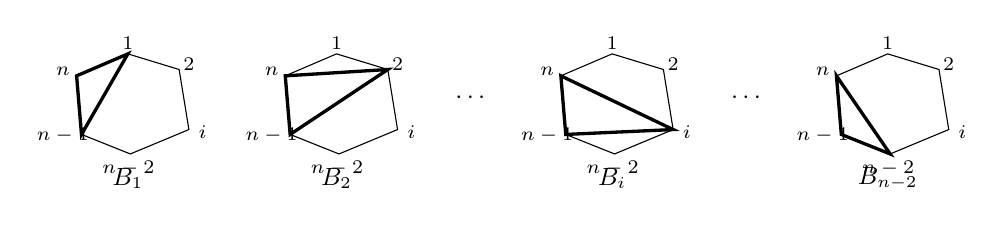
\begin{tikzpicture}[x=1cm,y=1cm,every node/.style={font=\small}]
  \newcommand{\splitpoly}[4]{%
    \begin{scope}[shift={(#1,#2)},scale=0.62]
      \coordinate (a) at (0,1.1);
      \coordinate (b) at (1.05,0.78);
      \coordinate (c) at (1.25,-0.45);
      \coordinate (d) at (0.05,-0.95);
      \coordinate (e) at (-0.95,-0.55);
      \coordinate (f) at (-1.05,0.65);
      \draw (a)--(b)--(c)--(d)--(e)--(f)--cycle;
      \draw[very thick] #3;
      \node at (0,-1.45) {#4};
      \node[font=\scriptsize] at ($(a)+(0,0.22)$) {\(1\)};
      \node[font=\scriptsize] at ($(b)+(0.20,0.10)$) {\(2\)};
      \node[font=\scriptsize] at ($(f)+(-0.28,0.10)$) {\(n\)};
      \node[font=\scriptsize] at ($(e)+(-0.38,-0.02)$) {\(n-1\)};
      \node[font=\scriptsize] at ($(d)+(-0.04,-0.30)$) {\(n-2\)};
      \node[font=\scriptsize] at ($(c)+(0.28,-0.05)$) {\(i\)};
    \end{scope}}
  \splitpoly{-4.0}{0}{(e)--(a)--(f)--cycle}{\(B_1\)}
  \splitpoly{-1.35}{0}{(e)--(b)--(f)--cycle}{\(B_2\)}
  \node at (0.35,0.12) {\(\cdots\)};
  \splitpoly{2.15}{0}{(e)--(c)--(f)--cycle}{\(B_i\)}
  \node at (3.85,0.12) {\(\cdots\)};
  \splitpoly{5.65}{0}{(e)--(d)--(f)--cycle}{\(B_{n-2}\)}
\end{tikzpicture}

\smallskip
\textit{Phân loại theo đỉnh thứ ba của tam giác chứa cạnh \((n-1,n)\).}
\end{center}

Gọi \(B_i\) là tổng số phương án thuộc loại \(i\), khi đó
\[
  A_n=\sum_{i=1}^{n-2} B_i. \tag{1}
\]

Có thể tính \(B_i\) như sau. Với phương án loại \(i\), đa giác \(n\) cạnh ban
đầu đã bị chia thành một đa giác \(i+1\) cạnh và một đa giác \(n-i\) cạnh.
Công việc tiếp theo gồm hai bước: chia đa giác \(i+1\) cạnh thành tam giác,
có \(A_{i+1}\) phương án; và chia đa giác \(n-i\) cạnh thành tam giác, có
\(A_{n-i}\) phương án. Để tiện biểu diễn, đặt \(A_2=1\). Khi đó
\[
  B_i=A_{i+1}A_{n-i}. \tag{2}
\]
Thay (2) vào (1), ta được
\[
  A_n
  =\sum_{i=1}^{n-2} A_{i+1}A_{n-i}
  =\sum_{i=2}^{n-1} A_iA_{n+1-i}. \tag{3}
\]

Vì thế, mô hình toán học của bài toán là:
\begin{quote}
Biết giá trị \(n\) và dãy \(A_2,A_3,A_4,\ldots\), trong đó
\[
  A_2=1,
\]
\[
  A_j=\sum_{i=2}^{j-1} A_iA_{j+1-i},\qquad j>2.
\]
Cần tìm \(A_n\).
\end{quote}

Dựa vào mô hình này, ta có thể lần lượt tính \(A_3,A_4,\ldots,A_n\) rất thuận
lợi.

Mô hình toán học của phương pháp truy hồi ngắn gọn hơn phương pháp tìm kiếm,
mức độ trừu tượng hóa cao hơn, và hiệu quả cũng cao hơn nhiều. Chương trình
truy hồi đã có thể xử lý dữ liệu cỡ trung bình: khi \(n<100\), thời gian không
quá một giây. Nhưng khi \(n\) rất lớn, nó vẫn còn chậm; với \(n=250\), cần
\(18.7\) giây trên máy 486DX2/80. Kết quả thử nghiệm xem ở
Phụ lục~\ref{app:tables}.

\subsection{Phương pháp hàm sinh}

Mô hình toán học của phương pháp trước đã loại bỏ nhiều nội dung không liên
quan đến yêu cầu bài toán. Nhưng đồng thời, bài toán chỉ yêu cầu \(A_n\), còn
phương pháp trên lại tính toàn bộ \(A_3,\ldots,A_n\). Có thể không tính
\(A_3,\ldots,A_{n-1}\) mà trực tiếp tính \(A_n\) từ \(n\) hay không? Sau đây
ta dùng mô hình toán học là hàm sinh để giải quyết vấn đề này.

Xem \(A_2,A_3,A_4,\ldots\) là các hệ số của một chuỗi lũy thừa và đặt
\[
  Y(x)=\sum_{i=2}^{+\infty} A_i x^i
      =A_2x^2+A_3x^3+\cdots. \tag{4}
\]
Nếu giải được \(Y(x)\), ta cũng tìm được \(A_n\).

Để tìm \(Y(x)\), xét giá trị \(Y(x)^2\):
\[
  Y(x)^2=\sum_{i=4}^{+\infty}
  \left[\sum_{j=2}^{i-2} A_jA_{i-j}\right]x^i.
\]
Mà
\[
  \sum_{j=2}^{i-2} A_jA_{i-j}=A_{i-1},
\]
nên
\[
  Y(x)^2=A_3x^4+A_4x^5+\cdots. \tag{5}
\]
Lấy (5) trừ \(x\) nhân (4), ta được
\[
  Y(x)^2-xY(x)+A_2x^3=0.
\]
Thay \(A_2=1\) và giải \(Y(x)\):
\[
  Y(x)=\frac{x\pm\sqrt{x^2-4x^3}}{2}
      =x\cdot\frac{1\pm\sqrt{1-4x}}{2}.
\]
Vì
\[
  \sqrt{1-4x}=1-2x-2x^2-4x^3-\cdots
\]
có các hệ số sau hằng số đều âm, trong khi \(A_i>0\), nên
\[
  Y(x)=x\cdot\frac{1-\sqrt{1-4x}}{2}. \tag{6}
\]

Trong đó
\[
  \sqrt{1-4x}
  =\sum_{k=0}^{+\infty} \binom{1/2}{k}(-4x)^k,
\]
với
\[
  \binom{1/2}{k}
  =\frac{\frac12(\frac12-1)(\frac12-2)\cdots(\frac12-k+1)}{k!}.
\]
Do đó
\[
\begin{aligned}
Y(x)
&=x\cdot
  \frac{1-\sum_{k=0}^{+\infty}\binom{1/2}{k}(-4x)^k}{2} \\
&=-\sum_{k=1}^{+\infty}
  \frac{(-4)^k}{2}\binom{1/2}{k}x^{k+1}.
\end{aligned}
\]
Từ hệ số của \(x^k\), suy ra
\[
\begin{aligned}
A_k
&=-\frac{(-4)^{k-1}}{2}\binom{1/2}{k-1} \\
&=\frac{1\cdot3\cdot5\cdots(2k-5)}{(k-1)!}\,2^{k-2} \\
&=\frac{1\cdot3\cdot5\cdots(2k-5)\cdot2\cdot4\cdot6\cdots(2k-4)}
        {(k-1)!(k-2)!} \\
&=\frac{(2k-4)!}{(k-1)!(k-2)!}
 =\frac{1}{k-1}\binom{2k-4}{k-2}.
\end{aligned}
\]

Vậy ta thu được mô hình toán học trực tiếp tính \(A_n\):
\begin{quote}
Biết giá trị \(n\),
\[
  A_n=\frac{1}{n-1}\binom{2n-4}{n-2}. \tag{7}
\]
Cần tìm \(A_n\).
\end{quote}

Khi giải, chỉ cần dùng công thức (7) để tính trực tiếp \(A_n\).

Trong ba mô hình toán học, mô hình này biểu diễn ngắn gọn nhất và có mức độ
trừu tượng hóa cao nhất. Hiệu quả giải bằng mô hình này cũng cao nhất. Khi
\(n=1000\), thời gian không quá \(1\) giây; khi \(n=5000\), chỉ cần \(14.7\)
giây trên máy 486DX2/80. Kết quả thử nghiệm xem ở Phụ lục~\ref{app:tables}.

Tìm kiếm là một phương pháp cơ bản nhất, được xây dựng trên một mô hình toán
học khá phức tạp. Đặc điểm của nó là có thể tìm ra từng phương án chia, nhưng
dùng cách này để tính tổng số phương án rõ ràng không đúng trọng tâm, nên
hiệu quả rất thấp. Phương pháp truy hồi được xây dựng trên mô hình dãy số; do
loại bỏ nhiều yếu tố không cần thiết, hiệu quả tăng mạnh và có tác dụng tốt
khi \(n\le 300\). Phương pháp dùng hàm sinh là một tối ưu hóa toán học của
phương pháp truy hồi; nó rút ra kết luận ngắn gọn hơn và thể hiện ưu thế rõ
rệt khi \(n>300\).

Từ phân tích trên có thể rút ra kết luận: mức độ trừu tượng hóa của mô hình
toán học càng cao thì hiệu quả của nó càng cao. Kết luận này rất dễ hiểu, vì
mức độ trừu tượng hóa càng cao thì những thành phần không liên quan đến vấn
đề trong mô hình càng ít, nên hiệu quả càng cao. Ngược lại, nếu mức độ trừu
tượng hóa chưa đủ cao, mô hình còn chứa nhiều thành phần không liên quan đến
vấn đề, thì hiệu quả sẽ thấp hơn.

\section{Khái quát và ứng dụng mô hình toán học}

Mô hình toán học có tính khái quát.

Mô hình toán học được xây dựng trên cơ sở bản chất của vấn đề, chứ không phải
trên hiện tượng bề ngoài của nó. Vì vậy, dù hai vấn đề nhìn bề ngoài không hề
liên quan, miễn là chúng có cùng bản chất thì có thể dùng cùng một mô hình
toán học để giải. Tuy nhiên, thấy được hai vấn đề có cùng bản chất không phải
là việc dễ. Điều đó đòi hỏi ta gạt bỏ hiện tượng bề ngoài, so sánh và phân
tích cẩn thận, rồi thiết lập quan hệ tương ứng giữa các vấn đề.

Tính khái quát của mô hình toán học có quan hệ chặt chẽ với mức độ trừu tượng
hóa của nó. Các mô hình khác nhau được xây dựng để giải cùng một bài toán có
thể có khả năng khái quát khác nhau.

Sau đây ta áp dụng mô hình toán học được xây dựng bằng hàm sinh cho một số
bài toán khác.

\paragraph{Bài toán đếm cây.}
Hãy tìm số cây nhị phân có \(n\) nút.

Gọi \(D_k\) là số cây nhị phân có \(k\) nút. Khi đó:
\begin{itemize}
  \item Nếu \(k=0\), đó là cây rỗng, chỉ có một cách.
  \item Nếu \(k>0\), cây nhị phân có thể được chia thành nút gốc, cây con
  trái có \(i\) nút, và cây con phải có \(k-1-i\) nút. Vì vậy, số cây nhị
  phân có \(k\) nút bằng tích của số cây nhị phân có \(i\) nút và số cây nhị
  phân có \(k-1-i\) nút, cộng trên mọi \(i\) có thể.
\end{itemize}

Viết phân tích trên thành công thức:
\[
  D_0=1,
\]
\[
  D_k=\sum_{i=0}^{k-1} D_iD_{k-1-i}.
\]
So sánh dãy \(A\) ở trên với dãy \(D\) ở đây, ta có
\[
  D_n=A_{n+2}.
\]
Vì thế, biến đổi nhẹ mô hình toán học (7), ta được
\[
  D_n=\frac{1}{n+1}\binom{2n}{n}. \tag{8}
\]
Đến đây, ta đã giải được bài toán này bằng mô hình ở trên. Bài toán này và
bài toán chia đa giác có cùng bản chất: quy luật đếm của chúng là như nhau,
nên có thể dùng cùng một mô hình toán học để giải.

Để mở rộng mô hình này thêm nữa, ta phân tích lại bài toán trước. Đánh số
một-một \(n\) nút của mỗi cây nhị phân sao cho thứ tự duyệt trước của mọi cây
đều là \(1,2,3,\ldots,n\). Vì thứ tự duyệt trước và thứ tự duyệt giữa xác
định duy nhất một cây nhị phân, nên thứ tự duyệt giữa của mỗi cây nhị phân
đều khác thứ tự duyệt giữa của các cây nhị phân khác. Nếu giống nhau, hai cây
ấy chính là cùng một cây.

Mặt khác, với một cây nhị phân có thứ tự duyệt trước đã xác định, thứ tự
duyệt giữa của nó có thể được sinh ra bằng quá trình đưa các phần tử của thứ
tự duyệt trước vào ngăn xếp rồi lấy ra khỏi ngăn xếp. Vì vậy, mô hình toán
học này lại có thể trực tiếp dùng để giải bài toán sau.

\paragraph{Bài toán tàu vào và ra khỏi ngăn xếp.}
Một đoàn tàu có \(n\) toa, được đánh số lần lượt là \(1,2,3,\ldots,n\). Mỗi
toa có hai cách chuyển động: vào ngăn xếp và ra khỏi ngăn xếp. Hỏi có bao
nhiêu hoán vị có thể của \(n\) toa sau khi ra khỏi ngăn xếp?

So sánh bài toán này với bài toán trước: trạng thái ban đầu của đoàn tàu
\((1,2,3,\ldots,n)\) chính là thứ tự duyệt trước của cây nhị phân; việc toa
tàu vào và ra khỏi ngăn xếp tương ứng với việc nút cây vào và ra khỏi ngăn
xếp; trạng thái đoàn tàu sau khi ra khỏi ngăn xếp chính là thứ tự duyệt giữa
của cây nhị phân.

Đặt hai bài toán cạnh nhau, không khó nhận thấy số hoán vị có thể sau khi
đoàn tàu ra khỏi ngăn xếp chính là số thứ tự duyệt giữa của cây nhị phân, tức
là số cây nhị phân.

Gọi \(E_n\) là số cách sắp xếp của \(n\) toa, khi đó
\[
  E_n=\frac{1}{n+1}\binom{2n}{n}. \tag{9}
\]
Vậy ta lại dùng cùng một mô hình toán học để giải được bài toán này.

Khi khái quát mô hình toán học sang bài toán đếm cây, ta chỉ so sánh các công
thức truy hồi tương tự, nên có thể nói đó là một phép khái quát đơn giản. Khi
khái quát sang bài toán tàu vào và ra khỏi ngăn xếp, ta xuất phát từ bài toán
đếm cây, đặt hai vấn đề tương ứng với nhau và phải phân tích logic nhiều hơn,
nên phức tạp hơn. Trên thực tế, việc khái quát và ứng dụng nhiều mô hình toán
học đều đòi hỏi phân tích cẩn thận.

Từ một bài toán ban đầu, bài toán chia đa giác, mô hình toán học
\[
  X_n=\frac{1}{n+1}\binom{2n}{n}
\]
được xây dựng. Trong công thức, nội dung cụ thể của việc chia đã bị lược bỏ
hoàn toàn, chỉ còn lại bản chất của vấn đề: đếm. Vì công thức biểu đạt nội
hàm thực chất của phương pháp đếm,
\[
  X_0=1,\qquad X_k=\sum_{i=0}^{k-1}X_iX_{k-1-i},
\]
nên nó có khả năng được áp dụng rộng rãi hơn cho một lớp bài toán.

Hãy xét lại mô hình toán học của phương pháp tìm kiếm trong bài toán chia đa
giác. Trong hai bài toán vừa nêu, mô hình tìm kiếm rõ ràng không còn thích
hợp. Nó chứa từng phương án chia cụ thể của đa giác và không thể hiện tốt bản
chất đếm của vấn đề, do đó ảnh hưởng đến khả năng khái quát của mô hình này.
Trong hai bài toán kia, không có khái niệm nào tương ứng với một phương án
chia đa giác cụ thể; vì thế mô hình tìm kiếm trở nên bất lực. Ngược lại, mô
hình dãy số và mô hình hàm sinh vẫn áp dụng được cho cả hai bài toán. Đó
chính là vì mô hình của hai phương pháp sau trừu tượng hơn, nên thuận lợi hơn
cho việc khái quát.

\section{Tổng kết}

Ba ví dụ trên đã minh họa đầy đủ tính hiệu quả, tính khái quát của mô hình
toán học, cũng như quan hệ giữa hai tính chất ấy với tính trừu tượng.

Mô hình toán học có tính hiệu quả. Mô hình được xây dựng từ vấn đề thực tế có
thể loại bỏ nội dung không liên quan, làm quan hệ trở nên rõ ràng, nhờ đó có
lợi cho việc nâng cao hiệu quả.

Mô hình toán học có tính khái quát. Sau khi một mô hình toán học được xây
dựng để giải vấn đề thực tế, nó thường có thể được áp dụng cho cả một lớp vấn
đề thực tế. Thoạt nhìn, bài toán chia đa giác và bài toán tàu vào ra ngăn xếp
không có liên hệ gì; nhưng thông qua việc hiểu mô hình, ta có thể phát hiện
hai bài toán có liên hệ nội tại chặt chẽ: chúng có thể được giải bằng cùng
một mô hình toán học.

Tính hiệu quả của mô hình toán học gắn chặt với tính trừu tượng của nó. Mô
hình toán học càng trừu tượng thì hiệu quả của nó càng cao. Tính khái quát
của mô hình toán học cũng gắn chặt với tính trừu tượng. Mô hình toán học càng
trừu tượng thì càng dễ được áp dụng rộng rãi.

\appendix
\section{Phụ lục: bảng thử nghiệm và chương trình}
\label{app:tables}

\subsection{Bảng 1: so sánh thời gian chạy của các chương trình thiết kế theo
ba mô hình toán học}

\begingroup
\scriptsize
\begin{verbatim}
n     Thoi gian chay (giay, 486/80)     Ket qua
      Tim kiem  Truy hoi  Ham sinh
5     0.0       0.0       0.0            5
8     0.1       0.0       0.0            132
10    0.6       0.0       0.0            1430
11    3.2       0.0       0.0            4862
12    16.8      0.0       0.0            16796
20              0.0       0.0            477638700
30              0.1       0.0            263747951750360
40              0.1       0.0            176733862787006701400
50              0.1       0.0            131327898242169365477991900
70              0.3       0.0            86218923998960285726185640663701108500
100             0.8       0.0            5774335806960135778218770060804285633402073162475661100
                                         0
150             3.1       0.0            3959313147057001992888490018878757680451363792611793474
                                         9025519709205419589642069387800
200             8.3       0.1            3249701714469247204061030419891100129328703540371004596
                                         9725655314584740305629299507691330189130411971857871567
                                         302000
250             18.7      0.1            2942109465114274900932013291224718543203864499126811120
                                         3317168783696949400211003928295831546272022257999617419
                                         625465614367577576739594354716172000
300             37.1      0.1            2833615951128645491952141298699350894649246764901164418
                                         2088598624691519032559650708037365499927532029654393447
                                         0696213221877124543336783231045268972258070292241625633
                                         99190436400
\end{verbatim}
\endgroup

\subsection{Bảng 2: thời gian chạy và kết quả của phương pháp hàm sinh trên dữ
liệu lớn}

\begingroup
\scriptsize
\begin{verbatim}
n     Thoi gian chay (giay, 486/80)  Ket qua
500   0.2   3392161481258547533436328676042834151806671371051948224646322289022038948
            4961666016394087658935561710828507304323072584219401165213694125111808676
            7433831117255251093952216676752181549754039254079009518747834466367785846
            2596953622134102520200986176150660638780745851952786342361786271048679068
            0000
1000  0.6   1282659123120329389992418907864563882089032052318971850610071333658659691
            7650636508971392269636384330131169530183206423519818758891241594708333432
            8015864565893550987852108368101709312590228295938009433241620526247192140
            9995611627511580863150740180266996754602824885598197887476283926138637334
            4807651604630045903721337776816153681064661207184425277845724281859993280
            9910085516200019191596126573215746216258241717105949596945086725752677939
            9630744193300422624617858972825189717428936822555053619495392164363039745
            4492990445740264272985056960596626000194076108609551836149060341111411420
            3867955760000
5000  14.7  1990533983292846325166673506454278003389272904305553280180872823100271211
            8767340856613205258009823911061689822819966058800117396543598135427586955
            9792778429614014690786606171171528320083045044671489924972047501523334246
            8138724573840895739739033811420784581508456866514843728085684023096771538
            1553578655967556776543982717552905537280360991836287529653206624959870630
            8121895633339730969725161266875649077021947002631530501156605401466085759
            7536352915369221824992631352492185831978570219673534486780746350434887270
            3806682765573357532768717863477686122111338669153041998736992669734521138
            4136884623921590225108813107833859413755075491924954296242363596594466667
            1446673358771831246640688142040703856338776629977766659654255268159378975
            1044519117369900869457690210352595228237709489430574007459436019028016411
            0038827696035585915387351199097375301331556293580890493918098622380755233
            3892680521693312997068069144010511282780445912971074861274051992834639631
            0561216451805165334432417634618203226858919012500057666732553341830111147
            0819533812120988010445061003160557018172554817337108394059108173915553582
            1737987646875652182998581745666283678405193386287633644237910478216042546
            3668803378393982395552054129650108630734033416898205271951432275542407693
            1819721455040492976792101947671393514768860471507412891459327520118017269
            6786877749972031468886291116599954859230193707272332890105705243614350673
            5132885611033291722431843274758902459024223795911169335414024073046732892
            7395645459224329052247990854644972024029972827331377313107196086221062765
            0188202833681955696454854968868373243539755357093842908311125187443209114
            0686683008816625997915385029705586103119596051190592857213107922653357349
            7461860596111378869832344698856089798444316515490995417460293855758521378
            0659674972152322112734313586718289148701156895171132685679870431003809667
            4186956424692388366951410846587759001196659372267179038623797279196316562
            3988309844128732444707420528465376060417840530884098880455141863912466417
            6032592842849445923263161630959760172685607996743155249441458740184540341
            6372467040622320018510892266507167328210681172963043341422470770335588144
            8203281065661300736427314789935878982943581444410274031000848491803374826
            2914234177331202318998592244539101401954666570026383034960883253619564875
            1981624029939353157525782759785276380074202722356998363216687878275696045
            9799214540286045928686781434155385008768086213261980678561187332233776048
            5664946553533366401151012142801380925362116746164301057451528028965946453
            9972118062862177079566215629850386783557684491180752622175613789741648825
            9143313542109632709368336593742684914689724272085005469649013886496227350
            8257492244688170498625618918459291917844876832932013180312437483376087705
            8196194803111496823543186375259372960899823055880506318903220600017289601
            4818245773092045746539907057236677380540322691698615959422148103261747037
            1581495719930597851695669555189979332882416754183716357001209090944294741
            4739729976104880382195071324370634650548082582843292378198930180928100582
            81353800000
\end{verbatim}
\endgroup

\subsection{Chương trình}

\paragraph{1. Bài toán chia đa giác: phương pháp tìm kiếm (\texttt{sousuo.pas}).}

\begingroup
\footnotesize
\begin{verbatim}
{$A+,B-,D-,E-,F-,G+,I-,L-,N-,O-,P-,Q-,R-,S-,T-,V+,X+,Y-}
{$M 16384,0,655360}
Program SouSuo;
Const
 Max=30;
Type
 TPara=record l,r:integer;end; {kieu khoang}
Var
 method:Longint; {tong so phuong an}
 Para:array[1..Max]of TPara; {nhom khoang}
  n:integer;
  time:Longint;

Function M(a,b:integer):integer;{kieu so nguyen lon}
begin if a<b then m:=b else m:=a;end;

Procedure Make; {tim kiem tat ca phuong an chia da giac}
Var i,j:integer;
  sp,lp1,lp2:integer;
 Function Connect:boolean; {kiem tra khoang moi co xung dot voi khoang cu khong}
 var i,j,k:integer;b1,b2:boolean;
 begin
  j:=para[sp].l;k:=para[sp].r;
  Connect:=true;
  for i:=1 to sp-1 do
    begin
     if (j=para[i].l)or(j=para[i].r) then continue;
     if (k=para[i].l)or(k=para[i].r) then continue;
     if ((j>para[i].l)and(j<para[i].r))xor
        ((k>para[i].l)and(k<para[i].r))
       then exit;
    end;
  Connect:=false;
 end;

 Function PreFalse:boolean; {kiem tra co xung dot khac khong}
 var i:integer;j,k:integer;
 begin
  prefalse:=false;j:=para[sp].l;
  if j<=2 then exit;
  for i:=1 to sp do
    if (para[i].l=j-1)or(para[i].r=j-1) then exit;
  k:=j;j:=k-2;
  for i:=1 to sp do
    if (para[i].l=j)and(para[i].r=k) then exit;
  PreFalse:=true;
 end;


 Function Pop:boolean;forward;

 Function Push:boolean; {day vao ngan xep}
 begin
  inc(sp);
  Para[sp].l:=lp1;Para[sp].r:=lp2;
  Push:=((lp1=1)and(lp2=n))or(lp1>n)or(lp2>n)or connect;
  if prefalse then
    begin Push:=true;pop;exit;end;
  inc(lp2);
  if lp2>n then
    begin inc(lp1);lp2:=lp1+2;end;
 end;

 Function Pop:boolean; {lay ra khoi ngan xep}
 begin
  if sp=0 then
    begin dec(sp);pop:=false;exit;end;
  lp1:=Para[sp].l;lp2:=para[sp].r;dec(sp);
  inc(lp2);
  if lp2>n then
    begin inc(lp1);lp2:=lp1+2;end;
  Pop:=(lp1>n)or(lp2>n);
 end;
begin
 sp:=0; {dat con tro dinh ngan xep bang 0}
 lp1:=1;lp2:=3;
 method:=0;

 while (sp>=0) do
 begin
  if Push then while pop do;
  if sp=n-3 then {thu duoc mot phuong an}
   begin
     method:=method+1;
     while pop do;
   end;
 end;
 writeln('Total: ',method);
end;


var i:integer;s:string;
BEGIN
 write('Input N: ');
 readln(n);{nhap so canh cua da giac}
 time:=MemL[$40:$6c];
 if n<3 then writeln('Total: 0')
   else if n=3 then writeln('Total: 1')
   else MAKE; {tim kiem tat ca phuong an chia da giac}
 writeln('Time: ',(Meml[$40:$6c]-time)/18.2:5:1);
  {xuat thoi gian da dung}
END.
\end{verbatim}
\endgroup

\paragraph{2. Bài toán chia đa giác: phương pháp truy hồi (\texttt{ditui.pas}).}

\begingroup
\footnotesize
\begin{verbatim}
{$A+,B-,D-,E-,F-,G+,I-,L-,N+,O-,P-,Q-,R-,S-,T-,V+,X+,Y-}
{$M 16384,0,655360}
Program DiTui;
Const
   Len=100;Max=300;
Type
  Th=array[-1..Len+1]of integer;{kieu so nguyen lon}
Var
 method:array[1..Max]of Th; {tong phuong an chia i-canh la method[i]}
 n:integer; {so canh da giac can tinh}
  time:Longint;

Function M(a,b:integer):integer; {lay gia tri lon hon}
begin if a<b then m:=b else m:=a;end;

Procedure Add(var a:Th;b:Th); {a:=a+b; a,b la kieu so nguyen lon}
var i,j:integer;
begin
 j:=0;
 a[-1]:=m(a[-1],b[-1]);
 for i:=0 to a[-1] do
   begin inc(j,a[i]+b[i]);
        a[i]:=j mod 10000; {moi phan tu integer luu 4 chu so thap phan}
       j:=j div 10000;
   end;
 if j<>0 then
   begin inc(a[-1]);a[a[-1]]:=j;end;
end;

Procedure Mul(a,b:Th;var c:Th); {c:=a*b; a,b,c la kieu so nguyen lon}
var i,j:integer;k:Longint;
begin
 fillchar(c,sizeof(Th),0);
 for i:=0 to a[-1] do
   begin
     k:=0;
     for j:=0 to b[-1] do
      if i+j<=Len then
      begin
        inc(k,longint(a[i])*b[j]+c[i+j]);
        c[i+j]:=k mod 10000;
        k:=k div 10000;
      end;
     inc(c[i+b[-1]+1],k);
   end;
 c[-1]:=a[-1]+b[-1];
 if c[c[-1]+1]<>0 then inc(c[-1]);
end;

Procedure OutHigh(a:Th); {xuat so nguyen lon}
var s:string[4];i,j:integer;
begin
 write('Total: ');
 j:=a[-1];write(a[j]);
 for i:=j-1 downto 0 do
   begin
    str(a[i],s);while s[0]<#4 do s:='0'+s;
    write(s);
   end;
 writeln;
end;
Procedure Make; {truy hoi tinh tong so phuong an chia da giac}
var i,j:integer;a:Th;
begin
 fillchar(method,sizeof(method),0);
 method[2,0]:=1;
 method[3,0]:=1;
 fillchar(a,sizeof(a),0);
 for i:=4 to N do
   for j:=1 to i-2 do
   begin
     mul(method[j+1],method[i-j],a);
     Add(method[i],a);
   end;
 OutHigh(method[n]);
end;


var i:integer;s:string;
BEGIN
 write('Input N: ');
 readln(n); {nhap so canh cua da giac}
 time:=MemL[$40:$6c];
 if n<3 then writeln('Total: 0')
   else MAKE;{truy hoi tinh tong so phuong an chia da giac}
 writeln('Time: ',(Meml[$40:$6c]-time)/18.2:5:1);
  {xuat thoi gian da dung}
END.
\end{verbatim}
\endgroup

\paragraph{3. Bài toán chia đa giác: phương pháp hàm sinh, xem
\texttt{muhanshu.pas}.}

\begingroup
\footnotesize
\begin{verbatim}
{$A+,B-,D-,E-,F-,G+,I-,L-,N+,O-,P-,Q-,R-,S-,T-,V+,X+,Y-}
{$M 16384,0,655360}
Program MuHanShu;
Const
   Len=1400;Max=6000;
Type
  Th=array[0..Len+1]of integer;{kieu so nguyen lon 1, luu theo chu so}
  Ty=array[0..Max]of integer;{kieu so nguyen lon 2, luu theo thua so}
Var
 fi,fo:text;fin,fon:string;
 n:integer;
 time:Longint;

Procedure Mul(var a:Th;b:integer); {a:=a*b; a la kieu so nguyen lon 1}
Var i:integer;k:Longint;
begin
 k:=0;
 for i:=1 to a[0] do
   begin
    k:=k+a[i]*longint(b);
    a[i]:=k mod 10000;
    k:=k div 10000;
   end;
 if k<>0 then
   begin inc(a[0]);a[a[0]]:=k;end;
end;

Function MaxPublic(a,b:integer):integer; {uoc chung lon nhat cua a,b}
var i:integer;
begin
 repeat
  a:=a mod b;
  if a=0 then break;
  b:=b mod a;
 until b=0;
 MaxPublic:=a+b;
end;


Procedure Divide(var k:Ty;h:integer);{k:=k div h; k la kieu so nguyen lon 2}
Var i,j:integer;
begin
 for i:=1 to k[0] do
  if k[i] mod h =0 then
     begin k[i]:=k[i] div h;
          if k[i]=1 then begin k[i]:=k[k[0]];dec(k[0]);end;
          exit;
     end;
 for i:=k[0] downto 1 do
  if MaxPublic(k[i],h)>1 then
   begin
     j:=MaxPublic(k[i],h);
     h:=h div j;k[i]:=k[i] div j;
     if k[i]=1 then begin k[i]:=k[k[0]];dec(k[0]);end;
     if h=1 then exit;
   end;
end;

Procedure translate(k:Ty;var a:Th);{a:=k; a la kieu so nguyen lon 1,
k la kieu so nguyen lon 2}
Var i:integer;
begin
 a[1]:=1;a[0]:=1;
 for i:=1 to k[0] do mul(a,k[i]);
end;

Procedure Make;{tinh tong so phuong an chia da giac theo cong thuc}
Var i,j:integer;k:Ty;a:Th;s:string[4];
begin
 k[0]:=n-2;
 for i:=1 to n-2 do k[i]:=(2*n-3-i);
 for i:=n-2 downto 2 do divide(k,i);
 divide(k,n-1);


 translate(k,a);


 write('Total: ');
 j:=a[0];write(a[j]);
 for i:=j-1 downto 1 do
   begin
    str(a[i],s);while s[0]<#4 do s:='0'+s;
    write(s);
   end;
 writeln;
end;


var i:integer;s:string;
BEGIN
 write('Input N(<=',Max,'): ');
 readln(n); {nhap so canh cua da giac}
 time:=MemL[$40:$6c];
 if n<3 then writeln('Total: 0')
   else MAKE; {tinh tong so phuong an chia da giac theo cong thuc}
 writeln('Time: ',(Meml[$40:$6c]-time)/18.2:5:1);
  {xuat thoi gian da dung}
END.
\end{verbatim}
\endgroup

\paragraph{4. Bài toán đếm cây và bài toán tàu vào ra ngăn xếp
(\texttt{tuiguang.pas}).}

\begingroup
\footnotesize
\begin{verbatim}
{$A+,B-,D-,E-,F-,G+,I-,L-,N+,O-,P-,Q-,R-,S-,T-,V+,X+,Y-}
{$M 16384,0,655360}
Program TuiGuang;
Const
   Len=1400;Max=5002;
Type
  Th=array[0..Len+1]of integer;{kieu so nguyen lon 1, luu theo chu so}
  Ty=array[0..Max]of integer;{kieu so nguyen lon 2, luu theo thua so}
Var
 fi,fo:text;fin,fon:string;
 n:integer;
 time:Longint;

Procedure Mul(var a:Th;b:integer); {a:=a*b; a la kieu so nguyen lon 1}
Var i:integer;k:Longint;
begin
 k:=0;
 for i:=1 to a[0] do
   begin
    k:=k+a[i]*longint(b);
    a[i]:=k mod 10000;
    k:=k div 10000;
   end;
 if k<>0 then
   begin inc(a[0]);a[a[0]]:=k;end;
end;

Function MaxPublic(a,b:integer):integer; {uoc chung lon nhat cua a,b}
var i:integer;
begin
 repeat
  a:=a mod b;
  if a=0 then break;
  b:=b mod a;
 until b=0;
 MaxPublic:=a+b;
end;

Procedure Divide(var k:Ty;h:integer);{k:=k div h; k la kieu so nguyen lon 2}
Var i,j:integer;
begin
 for i:=1 to k[0] do
  if k[i] mod h =0 then
     begin k[i]:=k[i] div h;
          if k[i]=1 then begin k[i]:=k[k[0]];dec(k[0]);end;
          exit;
     end;
 for i:=k[0] downto 1 do
  if MaxPublic(k[i],h)>1 then
   begin
     j:=MaxPublic(k[i],h);
     h:=h div j;k[i]:=k[i] div j;
     if k[i]=1 then begin k[i]:=k[k[0]];dec(k[0]);end;
     if h=1 then exit;
   end;

end;

Procedure translate(k:Ty;var a:Th);{a:=k; a la kieu so nguyen lon 1,
k la kieu so nguyen lon 2}
Var i:integer;
begin
 a[1]:=1;a[0]:=1;
 for i:=1 to k[0] do mul(a,k[i]);
end;

Procedure Make;{tinh theo cong thuc}
Var i,j:integer;k:Ty;a:Th;s:string[4];
begin
 k[0]:=n-2;
 for i:=1 to n-2 do k[i]:=(2*n-3-i);
 for i:=n-2 downto 2 do divide(k,i);
 divide(k,n-1);


 translate(k,a);


 write('Total: ');
 j:=a[0];write(a[j]);
 for i:=j-1 downto 1 do
   begin
    str(a[i],s);while s[0]<#4 do s:='0'+s;
    write(s);
   end;
 writeln;
end;


var i:integer;s:string;
BEGIN
 write('Input N(<=',Max-2,'): ');
 readln(n); {nhap N}
 inc(n,2);
 time:=MemL[$40:$6c];
 MAKE; {tinh theo cong thuc}
 writeln('Time: ',(Meml[$40:$6c]-time)/18.2:5:1);

   {xuat thoi gian da dung}
END.
\end{verbatim}
\endgroup

\section*{Tài liệu tham khảo}

\begin{enumerate}
  \item \emph{Olympic Tin học}, số 1--2 năm 1998, do Ủy ban phổ cập của Hội
  Máy tính Trung Quốc và Tsinghua University ACM Student Chapter chủ biên,
  trang 87 và 93--94.

  \item Yan Weimin và Wu Weimin, \emph{Cấu trúc dữ liệu}, tái bản lần thứ hai,
  Nhà xuất bản Đại học Thanh Hoa, tháng 6 năm 1992, trang 150--154.

  \item Kong Fanhai, \emph{Sách đọc mô hình hóa toán học cho học sinh trung
  học}, Nhà xuất bản Giáo dục Giang Tô, tháng 1 năm 1998.
\end{enumerate}

\end{document}
